\documentclass[border=2pt]{standalone}
\usepackage{tikz}
\usepackage{tikz-cd}
\begin{document}
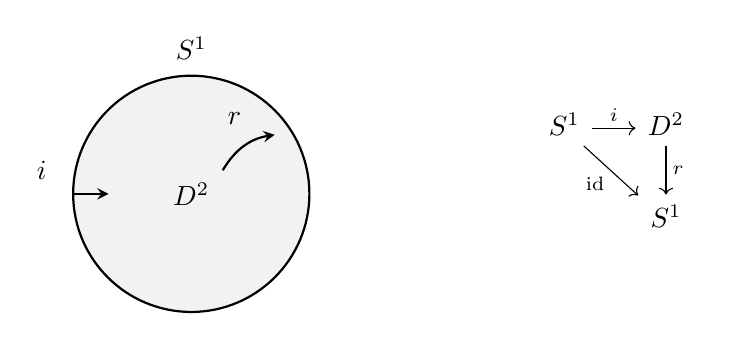
\begin{tikzpicture}[scale=1]
  % disk D^2 with boundary S^1, inclusion i, retraction r
  \begin{scope}
    \filldraw[fill=black!5,draw=black,thick] (0,0) circle (1.5);
    \node at (0,0) {$D^2$};
    \node at (0,1.85) {$S^1$};
    \draw[->,>=stealth,thick] (-1.5,0) -- (-1.05,0);
    \node at (-1.9,0.3) {$i$};
    \draw[->,>=stealth,thick] (0.4,0.3) to[bend left=25] (1.06,0.75);
    \node at (0.55,0.95) {$r$};
  \end{scope}

  % commutative triangle r o i = id
  \begin{scope}[xshift=5.4cm,yshift=0.3cm]
    \node {$
      \begin{tikzcd}[column sep=1.6em,row sep=1.8em]
        S^1 \arrow[r,"i"] \arrow[dr,"{\rm id}"'] & D^2 \arrow[d,"r"] \\
        & S^1
      \end{tikzcd}
    $};
  \end{scope}
\end{tikzpicture}
\end{document}
